\chapter{PWM Generation Figures} \label{A:PWM}

\section{Analogue PWM Generation} \label{A:analogue_PWM}


\begin{figure}[H]
    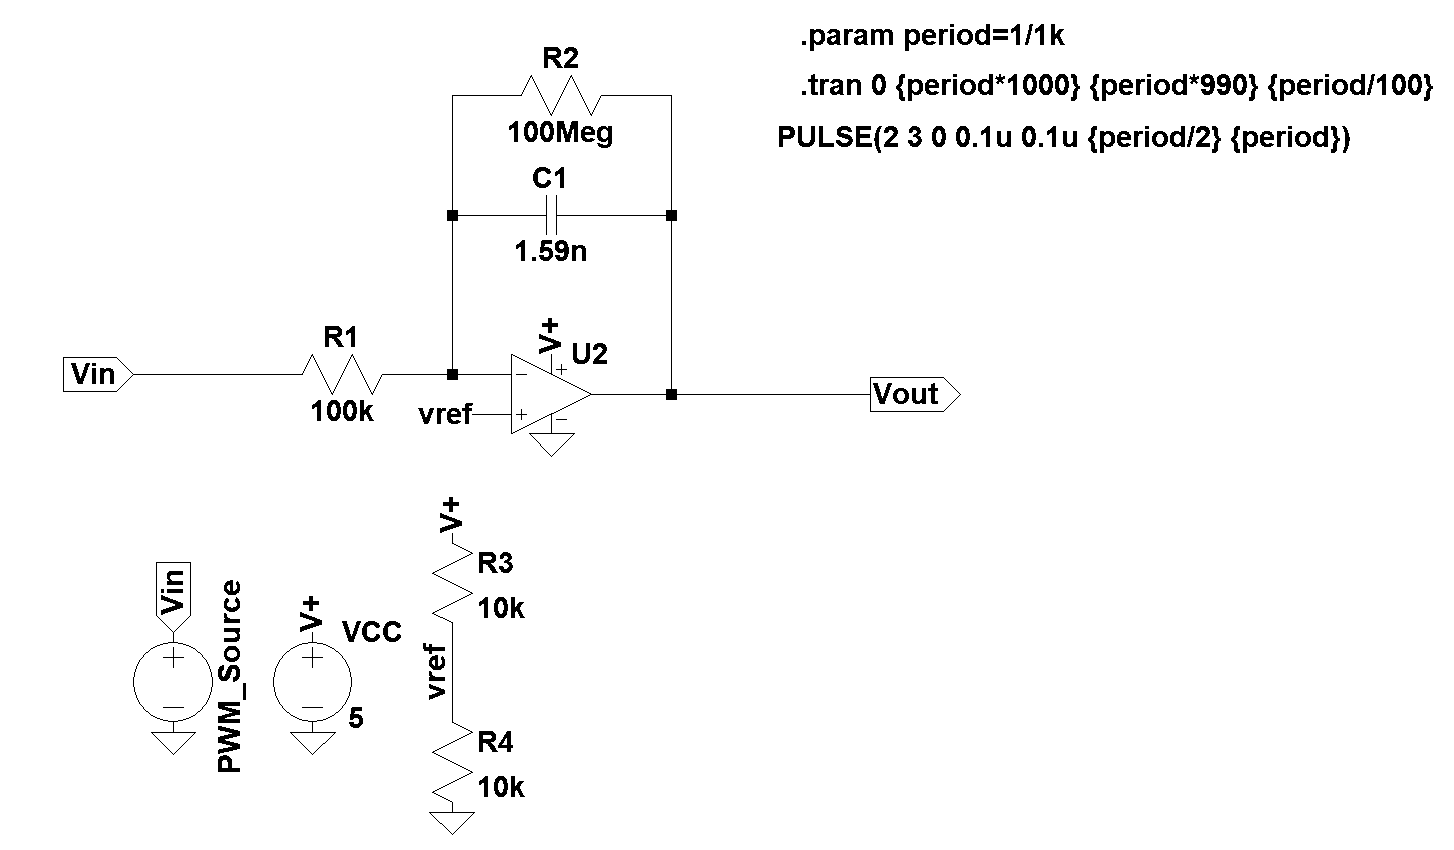
\includegraphics[width = 0.95\textwidth]{pwm/analog/analogue_PWM_ltspice_circuit.png}
    \caption{Operational amplifier integrator LTSpice circuit simulation}
\end{figure}

\begin{figure}[H]
    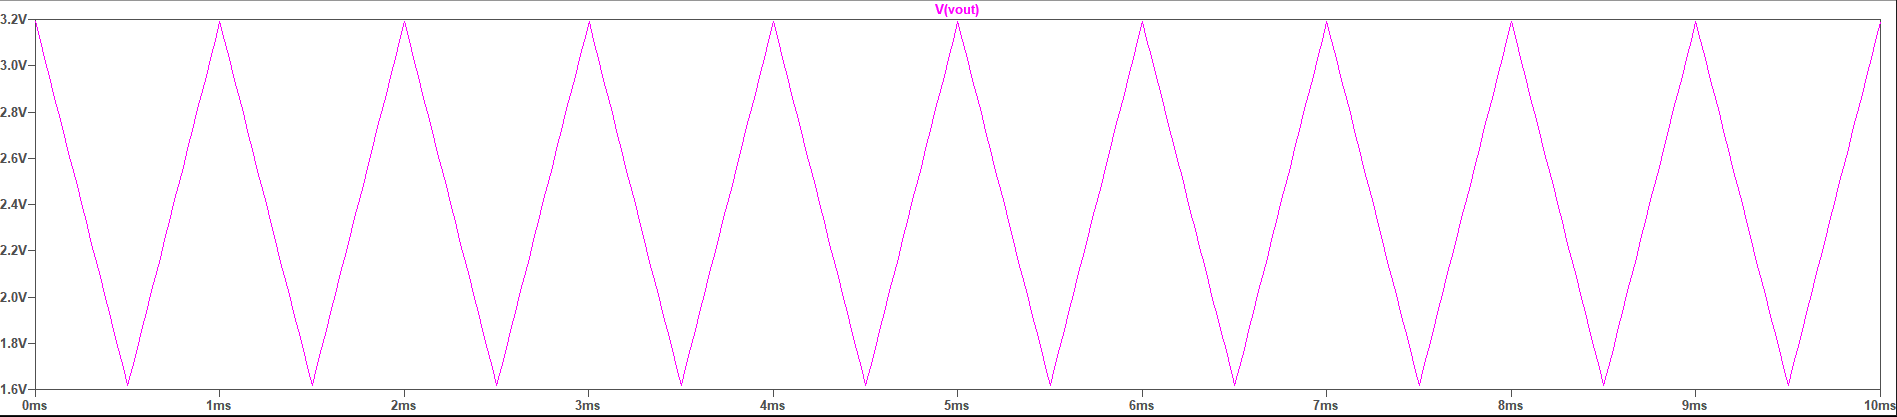
\includegraphics[width = 0.95\textwidth]{pwm/analog/analogue_PWM_ltspice_1k.png}
    \caption{Operational amplifier integrator simulation with a 1$kHz$ square wave input. Output triangle wave amplitude of 1.5V}
\end{figure}

\begin{figure}[H]
    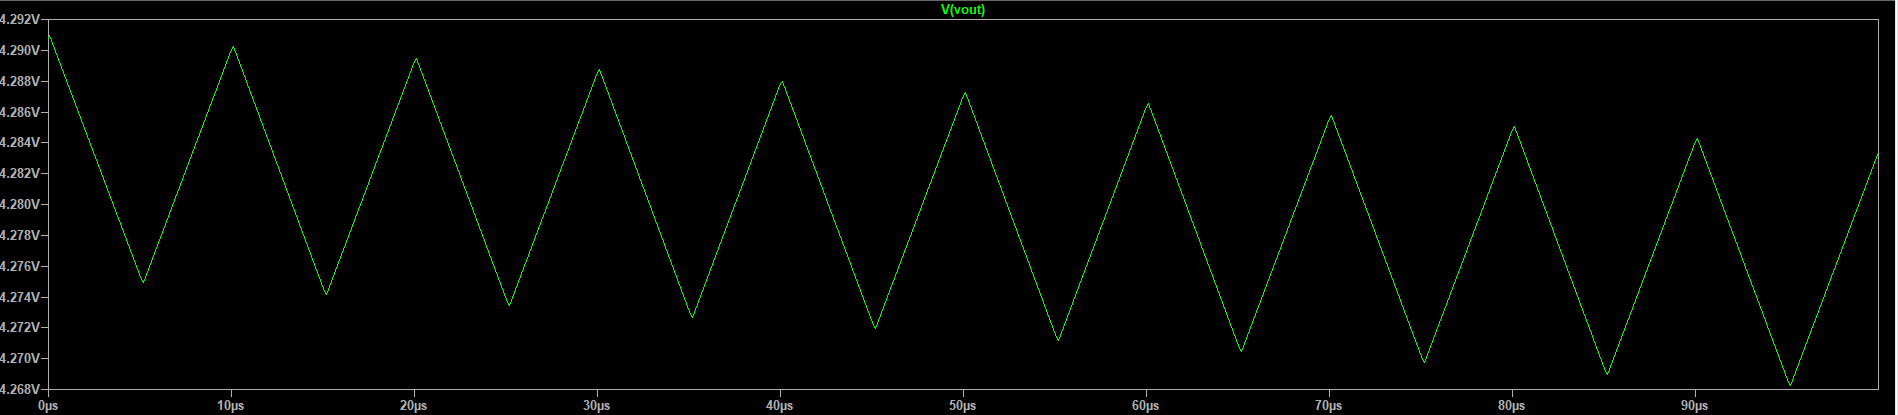
\includegraphics[width = 0.95\textwidth]{pwm/analog/analogue_PWM_ltspice_100k.png}
    \caption{Operational amplifier integrator simulation with a 1$kHz$ square wave input. Output triangle wave amplitude of 20mV}
\end{figure}


\section{Digital PWM Generation} \label{A:digital_PWM}

\begin{figure}[H]
    \centering
    \begin{subfigure}{0.45\textwidth}
        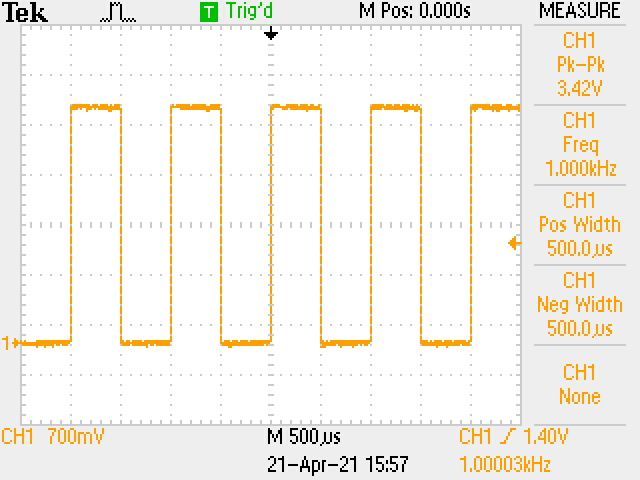
\includegraphics[width=\columnwidth]{pwm/duty/1kHz_50Duty.JPG}
        \subcaption{Digital PWM Generation at $1kHz$ and a 50\% duty cycle}

    \end{subfigure}
    \begin{subfigure}{0.45\textwidth}
        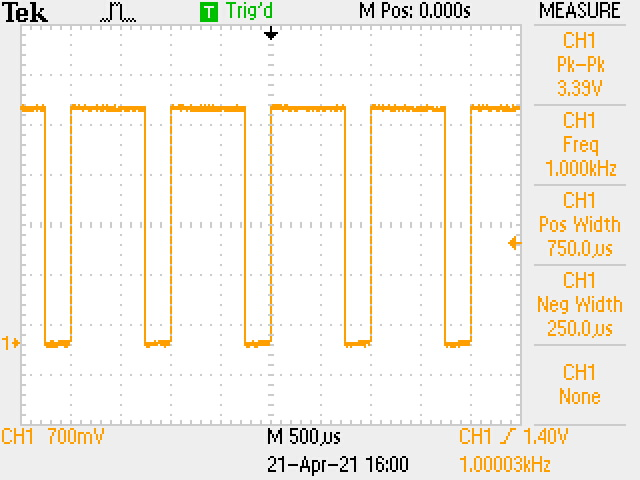
\includegraphics[width=\columnwidth]{pwm/duty/1kHz_75Duty.JPG}
        \subcaption{Digital PWM Generation at $1kHz$ and a 75\% duty cycle}

    \end{subfigure}
    \caption{Digital PWM Generation at $1kHz$}

\end{figure}

\begin{figure}[H]
    \centering
    \begin{subfigure}{0.45\textwidth}
        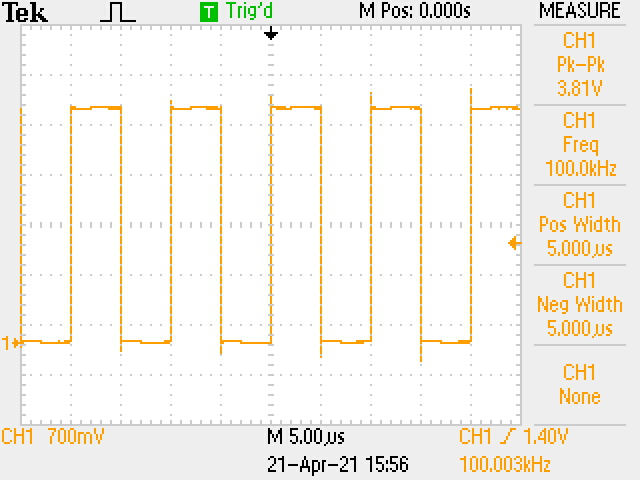
\includegraphics[width=\columnwidth]{pwm/duty/100kHz_50Duty.JPG}
        \subcaption{Digital PWM Generation at $100kHz$ and a 50\% duty cycle}

    \end{subfigure}
    \begin{subfigure}{0.45\textwidth}
        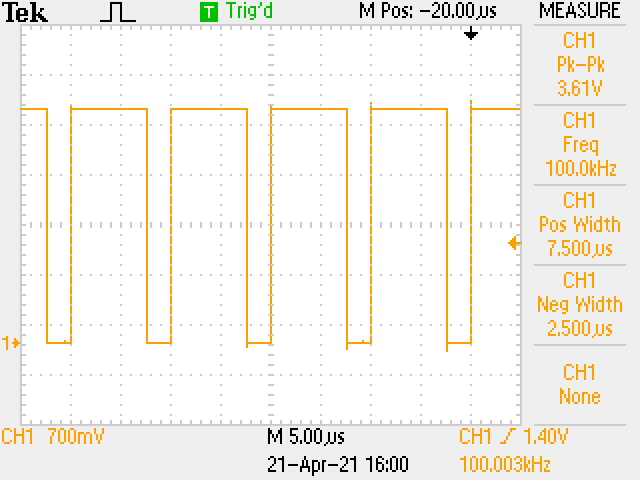
\includegraphics[width=\columnwidth]{pwm/duty/100kHz_75Duty.JPG}
        \subcaption{Digital PWM Generation at $100kHz$ and a 75\% duty cycle}

    \end{subfigure}
    \caption{Digital PWM Generation at $100kHz$}

\end{figure}